\chapter{Evolution of $V_{BE}$ with respect to temperature}

The details of the calculation of the dependence of $V_{BE}$ to temperature. We fisrt devellop the temperature dependence : 

\begin{align}
  V_{BE} & = \frac{k_BT}{q} \cdot ln \left( \frac{I_C}{I_S} \right) \\
  I_S ~   & \alpha ~ \mu ~ k T ~ n_i^2 \\
  \mu ~   & \alpha ~ \mu_0 ~ T^m \\
  n_i^2 ~ & \alpha~ T^3  \cdot  exp\left(\frac{E_g}{kT}\right)
\end{align}

With $\mu$ the mobility of the carriers, $n_i$ the intrinsic carrier concentration of silicon and $E_g~\approx 1.12 eV$ the bandgap energy of silicon.

We introduce a parameter b, which is a proprtionnality factor :

\begin{equation}
  I_S = b T^{4+m} \cdot exp\left(\frac{E_g}{kT}\right)
\end{equation}

Once we have devellop the expression with respect with T, we start to derivate the expression : 

\begin{equation}
    \frac{\partial V_{BE}}{\partial T} = \frac{\partial U_{T}}{\partial T}\cdot ln \left( \frac{I_C}{I_S} \right) + \frac{\partial I_{S}}{\partial T} \cdot \frac{U_T}{I_S}
\end{equation}

\begin{equation}
  \frac{\partial I_{S}}{\partial T} = b(4+m)T^{3+m}\cdot exp\left(\frac{E_g}{kT}\right) + bT^{4+m}\left(exp\left(\frac{E_g}{kT}\right)\right)\cdot \frac{E_g}{k T^{2}} 
\end{equation}

  
\begin{equation}
  \frac{U_T}{I_S} \frac{\partial I_{S}}{\partial T} = (4+m)\frac{U_T}{T} + \frac{E_g}{kT^2}\cdot U_T
\end{equation}

We obtain finally :

\begin{align}
  \frac{\partial V_{BE}}{\partial T} & = \frac{U_T}{T} ln \left( \frac{I_C}{I_S} \right) - (4+m)\frac{U_T}{T} - \frac{E_g}{kT^2}\cdot U_T \\
  \frac{\partial V_{BE}}{\partial T} & = \frac{V_{BE} - (4+m)U_T - E_g/q}{T}
\end{align}

\chapter{Output resistance of Beta Multiplier Current Source}

We can first draw the small signal schematic :

\begin{figure}[h]
  \begin{center}
    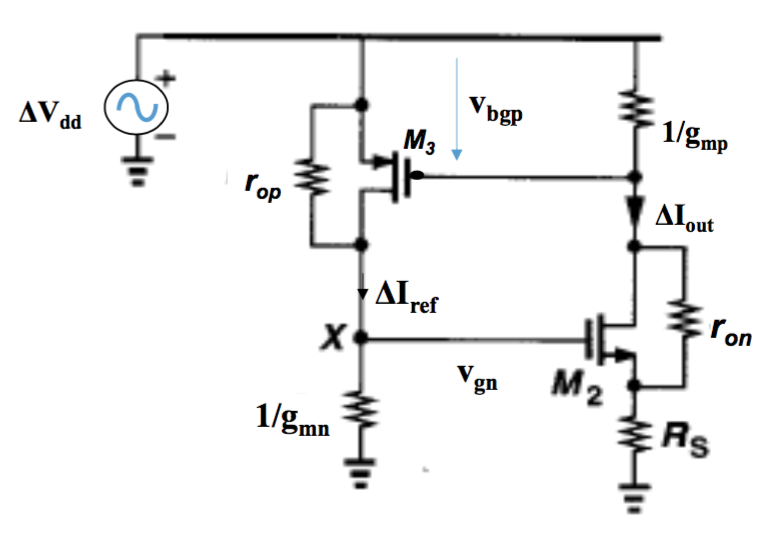
\includegraphics[scale=0.25]{photo/small_sig_bm}
  \end{center}
  \caption{Small Signal Analysis}
  \label{deltaiout}
\end{figure}

We have the in the right branch :

\begin{align}
  \Delta V_{DD} & = \frac{\Delta I_{out}}{g_{mp}} + R_s\cdot \Delta I_{out} + r_{on}\cdot ( \Delta I_{out} - g_{mn}(M2)\cdot v_{gn} + n \cdot g_{mn}(M2) \cdot R_S \Delta I_{out}  ) \\ 
  \Delta V_{DD} & \approx 3 \cdot r_{on} \Delta I_{out} - 2 \cdot r_{on} g_m v_{gn} 
\end{align}

We have the in the left branch :

\begin{align}
  \frac{\Delta V_{DD} - v_{gn}}{r_{op}} + g_{mp} \frac{\Delta I_{out}}{g_{mp}} & = g_{mn} v_{gn} \\ 
  g_{mn}~v_{gn} & \approx \frac{\Delta V_{DD}}{r_{op}} + \Delta I_{out}  
\end{align}

Finaly we have :

\begin{equation}
  \frac{\Delta I_{out}}{\Delta V_{DD}} \approx \frac{1}{r_{on}} + \frac{2}{r_{op}}
\end{equation}